

No se realizaron modificaciones al diseño E-R original; el diagrama se conserva tal cual. Las decisiones tomadas durante la traducción se detallan a continuación.\\ \\

\subsection*{Modelo Entidad-Relación}

\begin{figure}[H]
  \centering
 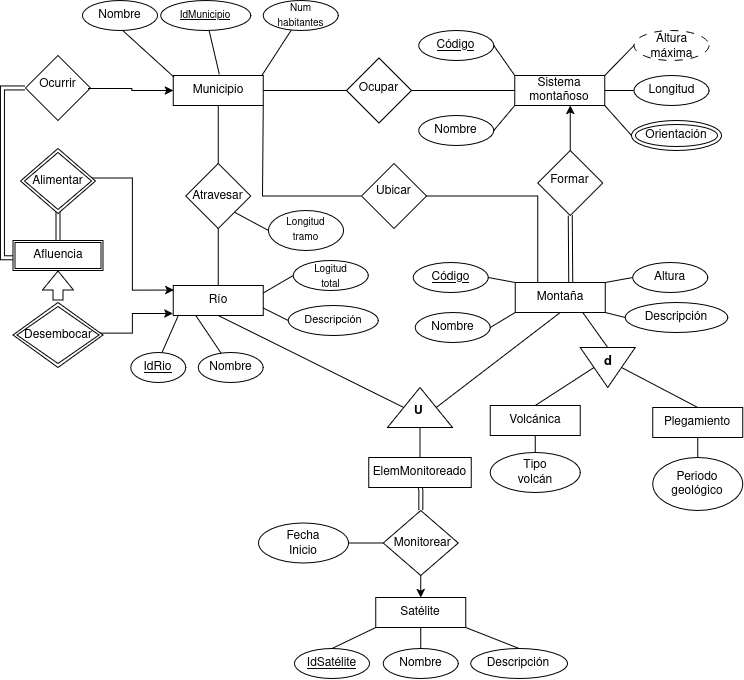
\includegraphics[width=\textwidth]{imagenes/Ejercicio2b(E-R).png}
  \caption{Modelo E-R del Sistema de Información Geográfica}
\end{figure}

\begin{figure}[H]
  \centering
 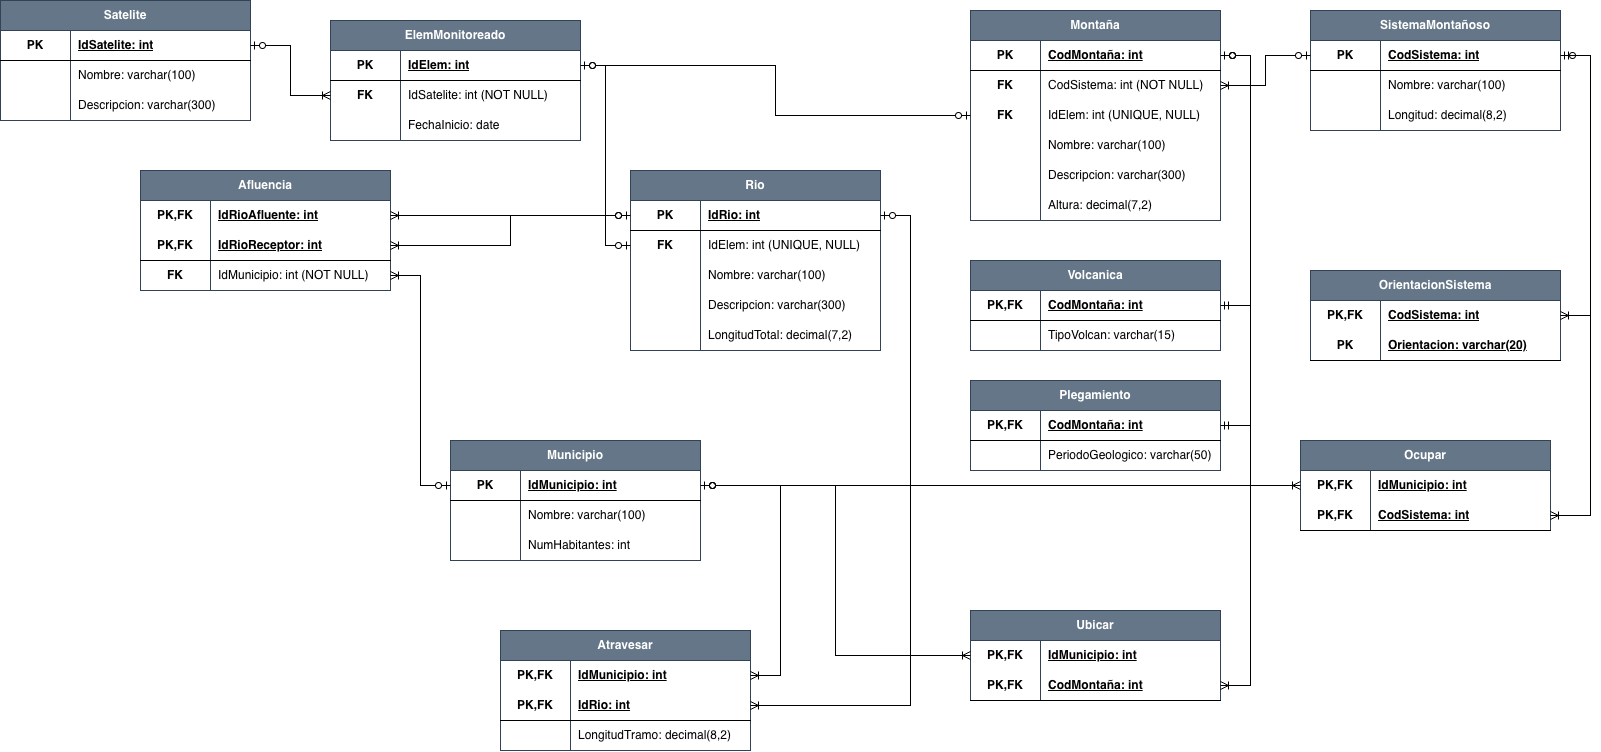
\includegraphics[width=\textwidth]{imagenes/Ejercicio2b(Relacional).png}
  \caption{Traducción al Modelo Relacional del Sistema de Información Geográfica}
\end{figure}

\subsection*{Traducción al Modelo Relacional}
\noindent
Los atributos de la llave primaria aparecen \pk{subrayados} y las llaves foráneas se marcan con el superíndice \textsuperscript{FK}.\\ \\
\textbf{Satelite}(\pk{IdSatelite},\ Nombre,\ Descripcion)\\ \\
\textbf{ElemMonitoreado}(\pk{IdElem},\ \fk{IdSatelite},\ FechaInicio)\\ \\
\textbf{Rio}(\pk{IdRio},\ \fk{IdElem},\ Nombre,\ Descripcion,\ LongitudTotal)\\ \\
\textbf{SistemaMontañoso}(\pk{CodSistema},\ Nombre,\ Longitud)\\ \\
\textbf{OrientacionSistema}(\pkfk{CodSistema},\ \pk{Orientacion})\\ \\
\textbf{Montaña}(\pk{CodMontaña},\ \fk{CodSistema},\ \fk{IdElem},\ Nombre,\ Descripcion,\ Altura)\\ \\
\textbf{Volcanica}(\pkfk{CodMontaña},\ TipoVolcan)\\ \\
\textbf{Plegamiento}(\pkfk{CodMontaña},\ PeriodoGeologico)\\ \\
\textbf{Municipio}(\pk{IdMunicipio},\ Nombre,\ NumHabitantes)\\ \\
\textbf{Atravesar}(\pkfk{IdMunicipio},\ \pkfk{IdRio},\ LongitudTramo)\\ \\
\textbf{Ubicar}(\pkfk{IdMunicipio},\ \pkfk{CodMontaña})\\ \\
\textbf{Ocupar}(\pkfk{IdMunicipio},\ \pkfk{CodSistema})\\ \\
\textbf{Afluencia}(\pkfk{IdRioAfluente},\ \pkfk{IdRioReceptor},\ \fk{IdMunicipio})


\subsection*{Restricciones de entidad}

\subsubsection*{Satelite}

\begin{longtable}{p{2.2cm} p{2.2cm} p{5.8cm} p{4.2cm} p{1.5cm}}
\toprule
\textbf{Atributo} & \textbf{Tipo} & \textbf{Dominio} & \textbf{Restricciones} & \textbf{Llave} \\
\midrule
\endfirsthead

\toprule
\textbf{Atributo} & \textbf{Tipo} & \textbf{Dominio} & \textbf{Restricciones} & \textbf{Llave} \\
\midrule
\endhead

\bottomrule
\endfoot


IdSatelite
& int
& Números mayores a 0
& NOT NULL (autoincremental)
& PK \\

Nombre
& varchar(100)
& Cadenas de hasta 100 caracteres.
& NOT NULL
&  \\

Descripcion
& varchar(300)
& Cadenas de hasta 300 caracteres.
& NULL permitido
&  \\

\end{longtable}


\subsubsection*{ElemMonitoreado}

\begin{longtable}{p{2.2cm} p{2.2cm} p{5.8cm} p{4.2cm} p{1.5cm}}
\toprule
\textbf{Atributo} & \textbf{Tipo} & \textbf{Dominio} & \textbf{Restricciones} & \textbf{Llave} \\
\midrule
\endfirsthead

\toprule
\textbf{Atributo} & \textbf{Tipo} & \textbf{Dominio} & \textbf{Restricciones} & \textbf{Llave} \\
\midrule
\endhead

\bottomrule
\endfoot


IdElem
& int
& Números mayores a 0
& NOT NULL (autoincremental)
& PK \\

IdSatelite
& int
& Números mayores a 0
& NOT NULL
& FK \\

FechaInicio
& date
& Fechas válidas con formato AAAA-MM-DD.
& NOT NULL
&  \\

\end{longtable}


\subsubsection*{Rio}

\begin{longtable}{p{2.6cm} p{2.2cm} p{5.8cm} p{4.2cm} p{1.5cm}}
\toprule
\textbf{Atributo} & \textbf{Tipo} & \textbf{Dominio} & \textbf{Restricciones} & \textbf{Llave} \\
\midrule
\endfirsthead

\toprule
\textbf{Atributo} & \textbf{Tipo} & \textbf{Dominio} & \textbf{Restricciones} & \textbf{Llave} \\
\midrule
\endhead

\bottomrule
\endfoot


IdRio
& int
& Números mayores a 0
& NOT NULL (autoincremental)
& PK \\

IdElem
& int
& Números mayores a 0
& NULL permitido;

UNIQUE
& FK \\

Nombre
& varchar(100)
& Cadenas de hasta 100 caracteres.
& NOT NULL
&  \\

Descripcion
& varchar(300)
& Cadenas de hasta 300 caracteres.
& NULL permitido
&  \\

LongitudTotal
& decimal(7,2)
& Números decimales mayores a 0
& NOT NULL;

Revisar: (LongitudTotal $>$ 0)
&  \\

\end{longtable}


\subsubsection*{SistemaMontañoso}

\begin{longtable}{p{2.2cm} p{2.2cm} p{5.8cm} p{4.2cm} p{1.5cm}}
\toprule
\textbf{Atributo} & \textbf{Tipo} & \textbf{Dominio} & \textbf{Restricciones} & \textbf{Llave} \\
\midrule
\endfirsthead

\toprule
\textbf{Atributo} & \textbf{Tipo} & \textbf{Dominio} & \textbf{Restricciones} & \textbf{Llave} \\
\midrule
\endhead

\bottomrule
\endfoot


CodSistema
& int
& Números mayores a 0
& NOT NULL (autoincremental)
& PK \\

Nombre
& varchar(100)
& Cadenas de hasta 100 caracteres.
& NOT NULL
&  \\

Longitud
& decimal(8,2)
& Números decimales mayores a 0
& NOT NULL;

Revisar: (Longitud $>$ 0)
&  \\

\end{longtable}


\subsubsection*{OrientacionSistema}

\begin{longtable}{p{2.2cm} p{2.2cm} p{5.8cm} p{4.2cm} p{1.5cm}}
\toprule
\textbf{Atributo} & \textbf{Tipo} & \textbf{Dominio} & \textbf{Restricciones} & \textbf{Llave} \\
\midrule
\endfirsthead

\toprule
\textbf{Atributo} & \textbf{Tipo} & \textbf{Dominio} & \textbf{Restricciones} & \textbf{Llave} \\
\midrule
\endhead

\bottomrule
\endfoot


CodSistema
& int
& Números mayores a 0
& NOT NULL
& PK, FK \\

Orientacion
& varchar(20)
& Cadenas dentro de la lista (Norte, Sur, Este, Oeste)
& NOT NULL;

Revisar que el valor sea uno en (Norte, Sur, Este, Oeste)
& PK \\

\end{longtable}


\subsubsection*{Montaña}

\begin{longtable}{p{2.2cm} p{2.2cm} p{5.8cm} p{4.2cm} p{1.5cm}}
\toprule
\textbf{Atributo} & \textbf{Tipo} & \textbf{Dominio} & \textbf{Restricciones} & \textbf{Llave} \\
\midrule
\endfirsthead

\toprule
\textbf{Atributo} & \textbf{Tipo} & \textbf{Dominio} & \textbf{Restricciones} & \textbf{Llave} \\
\midrule
\endhead

\bottomrule
\endfoot


CodMontaña
& int
& Números mayores a 0
& NOT NULL (autoincremental)
& PK \\

CodSistema
& int
& Números mayores a 0
& NOT NULL
& FK \\

IdElem
& int
& Números mayores a 0
& NULL permitido;

UNIQUE
& FK \\

Nombre
& varchar(100)
& Cadenas de hasta 100 caracteres.
& NOT NULL
&  \\

Descripcion
& varchar(300)
& Cadenas de hasta 300 caracteres.
& NULL permitido
&  \\

Altura
& decimal(7,2)
& Números decimales mayores a 0
& NOT NULL;

Revisar: (Altura $>$ 0)
&  \\

\end{longtable}


\subsubsection*{Volcanica}

\begin{longtable}{p{2.2cm} p{2.2cm} p{5.8cm} p{4.2cm} p{1.5cm}}
\toprule
\textbf{Atributo} & \textbf{Tipo} & \textbf{Dominio} & \textbf{Restricciones} & \textbf{Llave} \\
\midrule
\endfirsthead

\toprule
\textbf{Atributo} & \textbf{Tipo} & \textbf{Dominio} & \textbf{Restricciones} & \textbf{Llave} \\
\midrule
\endhead

\bottomrule
\endfoot

CodMontaña
& int
& Números mayores a 0
& NOT NULL
& PK, FK \\

TipoVolcan
& varchar(15)
& Cadenas de hasta 15 caracteres.
& NOT NULL
&  \\

\end{longtable}


\subsubsection*{Plegamiento}

\begin{longtable}{p{3.2cm} p{2.2cm} p{5.3cm} p{4.0cm} p{1.7cm}}
\toprule
\textbf{Atributo} & \textbf{Tipo} & \textbf{Dominio} & \textbf{Restricciones} & \textbf{Llave} \\
\midrule
\endfirsthead

\toprule
\textbf{Atributo} & \textbf{Tipo} & \textbf{Dominio} & \textbf{Restricciones} & \textbf{Llave} \\
\midrule
\endhead

\bottomrule
\endfoot


CodMontaña
& int
& Números mayores a 0
& NOT NULL
& PK, FK \\

PeriodoGeologico
& varchar(50)
& Cadenas de hasta 50 caracteres.
& NOT NULL
&  \\

\end{longtable}


\subsubsection*{Municipio}

\begin{longtable}{p{2.7cm} p{2.2cm} p{4.8cm} p{4.2cm} p{1.5cm}}
\toprule
\textbf{Atributo} & \textbf{Tipo} & \textbf{Dominio} & \textbf{Restricciones} & \textbf{Llave} \\
\midrule
\endfirsthead

\toprule
\textbf{Atributo} & \textbf{Tipo} & \textbf{Dominio} & \textbf{Restricciones} & \textbf{Llave} \\
\midrule
\endhead

\bottomrule
\endfoot


IdMunicipio
& int
& Números mayores a 0
& NOT NULL (autoincremental)
& PK \\

Nombre
& varchar(100)
& Cadenas de hasta 100 caracteres.
& NOT NULL
&  \\

NumHabitantes
& int
& Números enteros mayores o iguales a 0
& NOT NULL;

Revisar: (NumHabitantes $\geq$ 0)
&  \\

\end{longtable}


\subsubsection*{Atravesar}

\begin{longtable}{p{2.6cm} p{2.2cm} p{5.8cm} p{4.2cm} p{1.5cm}}
\toprule
\textbf{Atributo} & \textbf{Tipo} & \textbf{Dominio} & \textbf{Restricciones} & \textbf{Llave} \\
\midrule
\endfirsthead

\toprule
\textbf{Atributo} & \textbf{Tipo} & \textbf{Dominio} & \textbf{Restricciones} & \textbf{Llave} \\
\midrule
\endhead

\bottomrule
\endfoot


IdMunicipio
& int
& Números mayores a 0
& NOT NULL
& PK, FK \\

IdRio
& int
& Números mayores a 0
& NOT NULL
& PK, FK \\

LongitudTramo
& decimal(8,2)
& Números decimales mayores a 0
& NOT NULL;

Revisar: (LongitudTramo $>$ 0)
&  \\

\end{longtable}


\subsubsection*{Ubicar}

\begin{longtable}{p{2.2cm} p{2.2cm} p{5.8cm} p{4.2cm} p{1.5cm}}
\toprule
\textbf{Atributo} & \textbf{Tipo} & \textbf{Dominio} & \textbf{Restricciones} & \textbf{Llave} \\
\midrule
\endfirsthead

\toprule
\textbf{Atributo} & \textbf{Tipo} & \textbf{Dominio} & \textbf{Restricciones} & \textbf{Llave} \\
\midrule
\endhead

\bottomrule
\endfoot

IdMunicipio
& int
& Números mayores a 0
& NOT NULL
& PK, FK \\

CodMontaña
& int
& Números mayores a 0
& NOT NULL
& PK, FK \\

\end{longtable}


\subsubsection*{Ocupar}

\begin{longtable}{p{2.2cm} p{2.2cm} p{5.8cm} p{4.2cm} p{1.5cm}}
\toprule
\textbf{Atributo} & \textbf{Tipo} & \textbf{Dominio} & \textbf{Restricciones} & \textbf{Llave} \\
\midrule
\endfirsthead

\toprule
\textbf{Atributo} & \textbf{Tipo} & \textbf{Dominio} & \textbf{Restricciones} & \textbf{Llave} \\
\midrule
\endhead

\bottomrule
\endfoot


IdMunicipio
& int
& Números mayores a 0
& NOT NULL
& PK, FK \\

CodSistema
& int
& Números mayores a 0
& NOT NULL
& PK, FK \\

\end{longtable}


\subsubsection*{Afluencia}

\begin{longtable}{p{2.5cm} p{2.2cm} p{4.5cm} p{5.7cm} p{1.5cm}}
\toprule
\textbf{Atributo} & \textbf{Tipo} & \textbf{Dominio} & \textbf{Restricciones} & \textbf{Llave} \\
\midrule
\endfirsthead

\toprule
\textbf{Atributo} & \textbf{Tipo} & \textbf{Dominio} & \textbf{Restricciones} & \textbf{Llave} \\
\midrule
\endhead

\bottomrule
\endfoot


IdRioAfluente
& int
& Números mayores a 0
& NOT NULL
& PK, FK \\

IdRioReceptor
& int
& Números mayores a 0
& NOT NULL;

Revisar: (IdRioAfluente $\neq$ IdRioReceptor)
& PK, FK \\

IdMunicipio
& int
& Números mayores a 0
& NOT NULL
& FK \\

\end{longtable}